\documentclass[12pt]{article}
\usepackage{diagbox}
\usepackage{amsmath}
\usepackage{graphicx} %插入图片的宏包
\usepackage{float} %设置图片浮动位置的宏包
\usepackage{subfigure} %插入多图时用子图显示的宏包
\usepackage{setspace}
\usepackage{xeCJK}
\usepackage{amssymb}
\usepackage{biblatex}
\usepackage{enumerate}
\usepackage{multirow}
\usepackage[rightcaption]{sidecap}
\usepackage{caption}
\title{ A Bootstrap Approach to the Relationship between Taiwan's Unemployment Rate and Housing Prices }
\author{Ting-Chun Lin\thanks{
Undergraduate student in Department of Economics, National Taiwan University.\\ Email address: b09303097@ntu.edu.tw
}
} 


\date{June 2023}


\begin{document}

\maketitle

\begin{abstract}
{  
    This paper examines the relationship between high housing price and low unemployment rate in Taiwan. In this studies, I built an autoregressive distributed lag model to capture the effect of unemployment rate on housing price while holding Gross domestic product (GDP) and mortgage rate as control variables. Through inspecting data during 2000Q1-2022Q4 using Bootstrap method, the studies discover that during different time period, unemployment rate does not significantly influence housing price. The empirical results show that even when the macroeconomic condition unpredictably becomes dreadful, the effect of unemployment rate still insignificantly influenced housing price, which is different from Pavel (2018) that weak labor market explains the $\frac{1}{3}$ of house price decline.
    }
\end{abstract}
\textbf{Keywords:} Taiwan, Housing prices, Unemployment rate.
\newpage
\begin{spacing}{2}
\section{Introduction}
Ascending housing price has been an unresolved issue in Taiwan for the past twenty years. Starting from 2016, the growth of housing price has become more extreme. According to the articles,\footnote[1]{https://international.thenewslens.com/article/182910} in 2022, Taiwan's housing price is higher than countries like Norway whose GDP and minimum wages are both higher than Taiwan's.  Scholars have tried all means to identify the reasons for the phenomenon. Chu (2016) discussed how real estate transfer tax and other macroeconomic policies influenced Taiwan’s housing market. Chen(2020) dived into the question by analyzing Taiwan's public policy in housing financialization. These research indicates the dilemma the Taiwan house market facing is not a negligible issue. \\
\hspace*{1cm} In other aspect, in March 2023, the unemployment rate in Taiwan reached the bottom at about 3.6\% for the past 23 years.\footnote[2]{https://en.rti.org.tw/news/view/id/2009358}
From the view of Economics, unemployment rate is often considered as an important indicator to evaluate the macroeconomic conditions. M.M.H. Mukit, A.I. Abdel-Razzaq and M.S. Islam (2020) stated that GDP growth rate, inflation, and foreign direct investment flows have statistically significant impacts on unemployment rate both in short-run and long-run. When the unemployment rate is low, disposable income may increase, influencing individual decisions over investment. Beata (2022) indicated growing unemployment rate can be best explained by the deterioration of the overall situation on the labor market. Gintare, Olena, Despoina(2022) discussed how the macroeconomic condition including unemployment rate influences individual's well-being. To sum up, these papers elaborated how important unemployment rate is in the macroeconomic condition.\\ 
\hspace*{1cm} While the unemployment rate in Taiwan nearly remains steady in these 10 years, the housing price escalates at a dramatic rate. Whether  there is any mechanism behind the phenomenon is the purpose this paper intends to identify. The studies on relationship between housing price and unemployment rate have been done by other scholars. For example, Manuchehr Irandoust (2019) examines the causal linkages between real housing prices and unemployment rate using data from eight major European countries over the period of 1991-2016. The result differs in countries. In Italy, The Netherlands, Spain and Sweden, there is a unidirectional causality running from house prices to unemployment rate. While in Germany and Switzerland, the evidence indicates there is a bidirectional causality. And in the UK and France, there is no causality between the variables. It also emphasizes the stability of housing markets and house prices contributes to economic stability accompanied with stable unemployment rate.\\
\hspace*{1cm}Another example is Pavel Krivenko (2018). The paper investigates the link between unemployment rate and US housing market during the great recession. It uncovers that weak labor market explains $\frac{1}{3}$ of US house price decline. It also suggests that unemployment rate is signal of future income. When the unemployment is relatively high, expected future income is lowered, causing lower demand for housing in the bust.
In Ding (2022), the author used macroeconomic indicators such as unemployment rate, population, mortgage rate and so on to analyze the determinants of housing price, and the result shows that mortgage rates and unemployment rates will have a negative effect on housing price, which supports the statement that high unemployment rate may cause the housing price to fall. \\
\hspace*{1cm}In this paper, I will use quarterly data from 2000Q1 to 2022Q4 for Taiwan to investigate the impact of unemployment rate on housing price in different time period. Observing the trend of the unemployment rate, there are two ascending trend in 2000 and 2008 respectively. The paper will then discuss whether under these "tough" time, the effect has different interpretation. Ding (2022) states that mortgage rate will have a great harm on house prices. The increase of mortgage rate directly increases the housing loan pressure of home buyers, hindering the housing consumption demand. It also points out RGDP defined as the ratio of the ending GNP to the base GNP also plays an important role in housing price. If consumers have stronger spending power, their demand for house purchase will increase. Consequently, as the housing supply is fixed in the short term, the increasing demand will lead to the rise of house prices. Based on this, in order to clarify the real relationship, I will add other control variables including GDP and mortgage interest rate to capture the effects more precisely. In order to prevent the biasedness caused by the small sample size, Bootstrap method proposed by Bradley Efron will be applied to construct a more solid interpretation.
\newpage
\section{Research Method}
Following Ding (2022) and Manuchehr Irandoust (2019), I will build an autoregressive distributed lag (ARDL) model as follows:
\begin{equation}
\begin{split}
\Delta{\mathrm{HPI}}_{t} = \alpha_{t}+\beta_{t}\Delta{\log\mathrm{UR}}_{t}
+\gamma_{t}\Delta{\log\mathrm{IR}}_{t}+\eta_{t}\Delta{\log\mathrm{GDP}}_{t}+\sum_{j=1}^{k}\delta_{1,j}\Delta{\mathrm{HPI}}_{t-j}\\
+\sum_{j=1}^{k}\delta_{2,j}\Delta{\log\mathrm{UR}}_{t-j}+\sum_{j=1}^{k}\delta_{2,j}\Delta{\log\mathrm{IR}}_{t-j}+
\sum_{j=1}^{k}\delta_{2,j}\Delta{\log\mathrm{GDP}}_{t-j}+\varepsilon_{t}.
\end{split}
\end{equation} 
\hspace*{0.5cm}In equation (1) , HPI represents the housing price index, UR denotes the unemployment rate, IR indicates the mortgage interest rates as control variables, GDP shows the GDP as control variables and $\varepsilon$ is the white noise error term. $t$ is the time period($t $= 2000Q1,...,2022Q4).
The reason to include GDP as control variable is to fix the economy condition since GDP affects the macroeconomic condition to a great extent. As for mortgage interest rate, it directly affects housing demand and therefore influences housing price.\\
\hspace*{0.5cm}To determine how many lagged terms to be chosen, Akaike Information Criterion (AIC) will be applied. Since non-stationary time series data may cause biased result, to prevent this problem, I will first take difference on the HPI, and take log difference on UR, IR, and GDP. Unit root test will also be implemented to check stationarity.\\
\hspace*{0.5cm}Does economic condition play an important role in the relationship between unemployment rate and the housing prices is what I am interested in. According to Pavel Krivenko (2018), when the economic condition becomes worse, unemployment rate rises and causes people's expected future income to be lower, people tend to invest less than before. The housing price should fall.
\hspace*{0.5cm}Therefore, I will use the model to test different period to investigate the relationship between unemployment rate and housing price in different time period. The chosen time periods are (I) 2000Q1-2003Q3, (II) 2003Q4-2008Q2, (III) 2008Q3-2010Q3 and (IV) 2010Q4-2022Q4. (I) and (III) are the time period that we are interested in, since the unemployment rate are unusual high in these two periods. The former time phase is commonly considered the result of  structural change in Taiwan's industries, while the latter is due to the 2008 financial crisis. The expected result is to observe $\beta_t < 0$ in these two samples, which means when the unemployment rate rises, the housing price may fall.\\
\hspace*{0.5cm}Since there are only 92 observations in this study, the small sample biasedness may occur. To solve the dilemma, I will use the ARDL defined in equation (1) and resort to Bootstrap method to obtain the actual distribution of variables interested.
\section{Data}
Figure 1 shows the unemployment rate (monthly) in Taiwan from 2000M1 to 2022M12 collected from National Statistics, R.O.C. (Taiwan). Figure 2 shows the housing price index (seasonal) in Taiwan from 2000Q1 to 2022Q4 collected from Ministry of Interior. Figure 3 shows the GDP in USD from 2000Q1-2022Q4 collected from National Statistics, R.O.C. (Taiwan). Figure 4 shows the interest rate from 2000Q1-2022Q4 using the mortgage rate in the five main banks of Taiwan.
Table 1 shows the brief statistics of the variables.

\begin{figure}[H] %H为当前位置,!htb为忽略美学标准,htbp为浮动图形
\centering %图片居中
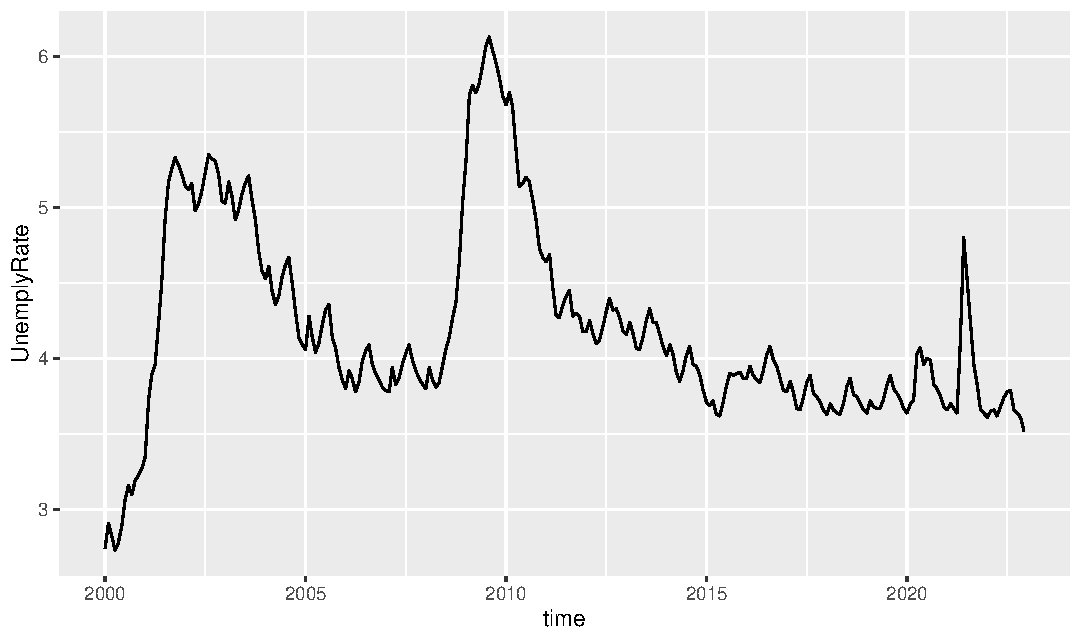
\includegraphics[width=1\textwidth]{unemploymentRate.pdf} %插入图片,[]中设置图片大小,{}中是图片文件名
\caption{Unemployment Rate from 2000-2022} %最终文档中希望显示的图片标题
\label{Fig.main1} %用于文内引用的标签
\end{figure}

\begin{figure}[H] %H为当前位置,!htb为忽略美学标准,htbp为浮动图形
\centering %图片居中
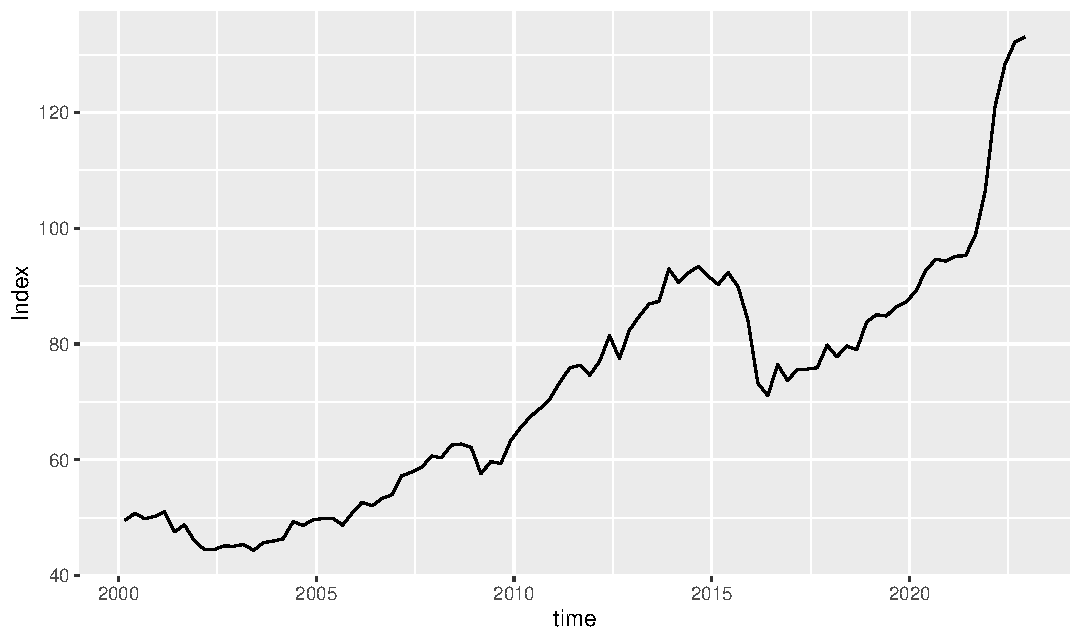
\includegraphics[width=1\textwidth]{houseIndex.pdf} %插入图片,[]中设置图片大小,{}中是图片文件名
\caption{Housing Price Index from 2000-2022} %最终文档中希望显示的图片标题
\label{Fig.main2} %用于文内引用的标签
\end{figure}

\begin{figure}[H] %H为当前位置,!htb为忽略美学标准,htbp为浮动图形
\centering %图片居中
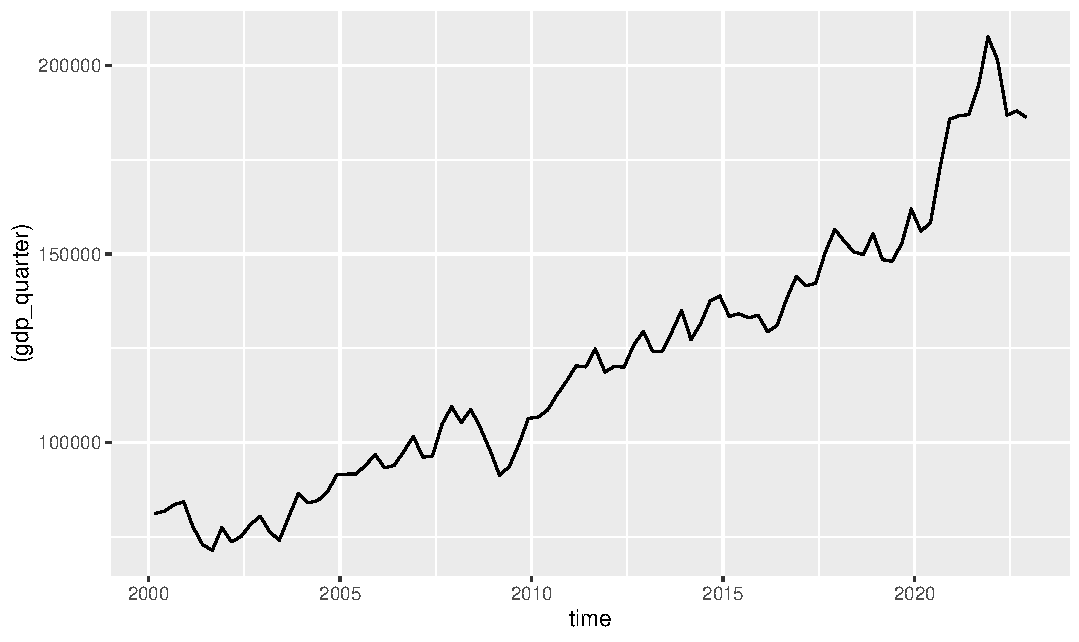
\includegraphics[width=1\textwidth]{GDP.pdf} %插入图片,[]中设置图片大小,{}中是图片文件名
\caption{GDP from 2000-2022} %最终文档中希望显示的图片标题
\label{Fig.main3} %用于文内引用的标签
\end{figure}

\begin{figure}[H] %H为当前位置,!htb为忽略美学标准,htbp为浮动图形
\centering %图片居中
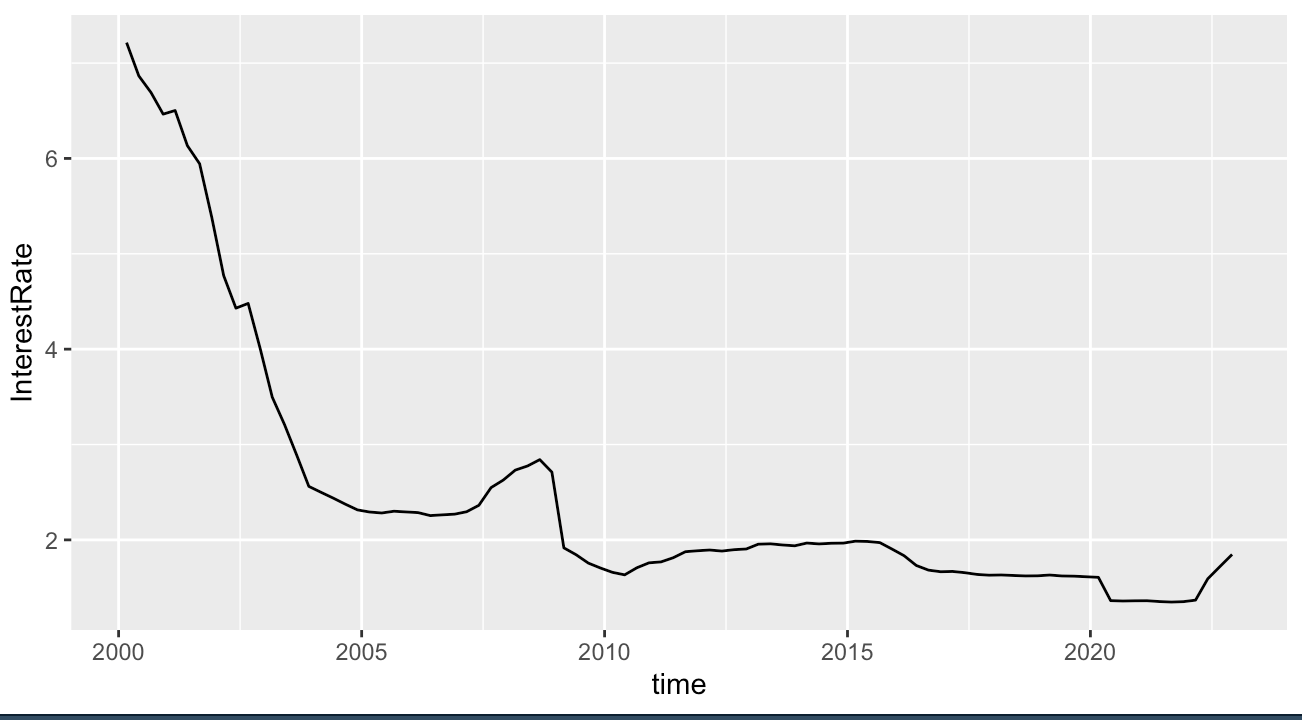
\includegraphics[width=1\textwidth]{截圖 2023-06-06 下午3.11.29.png} %插入图片,[]中设置图片大小,{}中是图片文件名
\caption{Interest Rate from 2000-2022} %最终文档中希望显示的图片标题
\label{Fig.main4} %用于文内引用的标签
\end{figure}



\begin{table}[h!]
\centering
\begin{tabular}{|l|l|l|l|l|}
\hline
Variable              & Mean     & Standard Deviation & Min   & Max    \\ \hline
Unemployment Rate(\%) & 4.192319 & 0.6483698          & 2.8   & 6.08   \\ \hline
House Index           & 71.69761 & 21.07596           & 44.36 & 133.06 \\ \hline
GDP(million USD)      & 121178.6 & 34719              & 71407 & 207602 \\ \hline
Interest Rate(\%)     & 2.460123 &  1.395632            &  1.348    & 7.215   \\ \hline
\end{tabular}
\caption{Statistics of variables}
\label{table:1}
\end{table}
To prevent the inference to be inaccurate, I take difference and log difference on the variables, and the Augmented Dickey-Fuller(ADF) test has been implemented to check the stationarity of the statistics. The ADF test statistics is presented in table 2. The results indicated that the variables we applied are stationary.
\begin{table}[h!]
\centering
\begin{tabular}{|l|l|l|l|l|}
\hline
Variable&$\Delta{\mathrm{Index}}$& $\Delta{\mathrm{\log(Unemply)}}$ &$\Delta{\log\mathrm{GDP}}$&$\Delta{\log\mathrm{IR}}$    \\ \hline
Z-statistics& -7.07 & -6.84& -8.369&  -6.322   \\ \hline
\end{tabular}
\caption{ADF Statistics of variables}
\label{table:2}
\end{table}
\newpage
\section{Empirical Result}
After obtaining all the data sets needed, I first simply run the ARDL model defined in equation (1). The decision on the lag terms is determined by Akaike Information Criterion (AIC).  The empirical result is shown in Table 3.
\begin{center}
\begin{tabular}{ |p{3.5cm}||p{2.5cm}|p{2.5cm}|p{2.5cm}| p{2.5cm}|  }
 \hline
Variable & 2000Q1-2003Q3 &2003Q4-2008Q2 &2008Q3-2010Q3&2010Q4-2022Q4  \\
 \hline
 $\Delta{\mathrm{Index}_{t-1}}$  & -0.49(0.27)   &-0.38(0.26)&  -0.65*(0.16)&0.36*(0.17)\\
 $\Delta{\mathrm{\log(Unemply)_t}}$&  1.81 (9.51) &  -8.58 (8.66)    &-19.42*(5.26)& -14.26 (12.58)      \\
 $\Delta{\mathrm{\log(Unemply)_{t-1}}}$ & -9.84 (6.68)  &- & - & -18.84  (12.85)\\
 $\Delta{\log\mathrm{GDP}}_{t}$   &6.86(7.82) &-9.95 (8.04)  &  -9.98(8.04)&  25.65(15.29)\\
$\Delta{\log\mathrm{GDP}}_{t-1}$&-& -&26.04(9.01)&-\\
$\Delta{\log\mathrm{IR}}_{t}$&  8.64(12.18)  &   -4.09(13.59)   &7.26(2.80) &2.22(17.09) \\
 Constant& 0.35(1.11)   &  1.34* (0.45)& 2.18**(0.32)& 0.33(0.59) \\ \hline
\end{tabular}
\captionof{table}{Empirical Result (without Bootstrap)}    
\end{center}
The result from table 3 shows that in 2008Q3-2010Q3, where the financial crisis took place, the influence of the unemployment rate significantly affects the housing price. However, it is not significant in other time period. Comparing with 2000Q1-2003Q3, where the structural change of Taiwan's industry began, there both exists peaks of unemployment rate in the era, while the impact of unemployment rate on housing price in 2008 financial crisis seems to be more considerable. \\
\hspace*{0.5cm}To explain the phenomenon, a possible account is that during 2001Q1-2003Q3, due to the structural change of Taiwan industry, the rise of unemployment rate is somehow predictable, people would try to reduce their  investment in a smoother way. While the 2008 financial crisis is much more unpredictable, the unemployment rate rocketing, causing the demand of real estate to respond dramatically.\\
\hspace*{0.5cm}However, if we simply take the result as conclusion, the issue of small data size might lead us to the spurious result. In order to tackle the problem, the Bootstrap method proposed by Bradley Efron is applied. I use the regression model from equation (1) and run 1000 bootstrap tests in each time period. By implementing the Bootstrap method, the construction of the distribution would be more solid. The corrected result is shown in table 4.
\begin{center}
\begin{tabular}{ |p{3.5cm}||p{2.5cm}|p{2.5cm}|p{2.5cm}| p{2.5cm}| }
 \hline
Variable & 2000Q1-2003Q3 &2003Q4-2008Q2 &2008Q3-2010Q3&2010Q4-2022Q4  \\
 \hline
 $\Delta{\mathrm{Index}_{t-1}}$  & -0.49(0.89)   &-0.38(0.29)&  -0.65(0.90)&0.36(0.26)\\
 $\Delta{\mathrm{\log(Unemply)_t}}$&  1.81 (38.86) &  -8.58 (9.58)    &-19.42(35.47)& -14.26 (11.82)      \\
 $\Delta{\mathrm{\log(Unemply)_{t-1}}}$ & -9.84 (22.58)  &- & - & -18.84  (18.62)\\
 $\Delta{\log\mathrm{GDP}}_{t}$   &6.86(26.99) &-9.95 (12.82)  &  -9.98(49.93)&  25.65(15.93)\\
$\Delta{\log\mathrm{GDP}}_{t-1}$&-& -&26.04(38.72)&-\\
$\Delta{\log\mathrm{IR}}_{t}$&  8.64(62.47)  &   -4.09(28.76)   &7.26(50.55) &2.22(30.16) \\
 Constant& 0.35(5.63)   &  1.34* (0.61)& 2.18(2.08)& 0.33(0.65)\\
 \hline
\end{tabular}
\captionof{table}{Empirical Result (with Bootstrap correction)}    
\end{center}
As table 4 presents, unemployment rate does not show significant impact on housing price in any time period, which disproves the previous statement that in poor economic conditions, the impact of unemployment rate affects housing price. The reason causing the difference may be contributed to the small sample size we used in the previous regression.
\newpage


\newpage
\section{Conclusion}
Taiwan's high housing price has grasped a lot of attention all over the world, the mechanism behind the phenomenon is somewhat more appealing. This paper examines the housing price from the labor supply perspective. The competitiveness of the labor market influences the expected labor income directly, and income impacts individual's decision. As expected income increases, people would increase their investment and hence cause the demand to rise, bidding up the housing price. Unemployment rate often be regarded as an important indicator of the labor market competitiveness, and therefore may be a well-explanatory variable.  \\
\hspace*{0.5cm} After controlling the GDP and the mortgage rate, the empirical result using Bootstrap method shows that there is insignificant relationship between unemployment rate and the housing price, even in the poor economic condition. The reason might be the low unemployment rate in Taiwan, even in the poor economic condition, the highest peek was only 6.08\% in the 2008 financial crisis, which is relatively low comparing to the U.S.A.'s 9.5\%. In other time period, there is no sharp volatility overall, making unemployment explanatory power weak on soaring housing price.\\
\hspace*{0.5cm}This paper mainly focus on the impact of single variable, I did not take the reaction of the variables into consideration. However in the real world, the reaction between macroeconomic variables may be more complicated, not taking these effects may lead to incorrect result. In further studies, vector autoregression model should be applied to catch the influence more precisely.


\newpage
\begin{thebibliography}{1}
%Irandoust, Manuchehr. (2019). House Prices and Unemployment: An Empirical Analysis of Causality. International Journal of Housing Markets and Analysis. 12. 148-164. 10.1108/IJHMA-03-2018-0021.
\bibitem{Irandoust, Manuchehr}
    Irandoust, Manuchehr. (2019).\emph{House Prices and Unemployment: An Empirical Analysis of Causality},
    International Journal of Housing Markets and Analysis. 12. 148-164. 
%Shiou-Yen Chu,
\bibitem{chu}
    Shiou-Yen Chu (2018).\emph{Macroeconomic policies and housing market in Taiwan},
    International Review of Economics \& Finance,Volume 58, 404-421,

 %Mukit, Mohammad Mushfiqul Haque and Abdel-Razzaq, Assim Ibrahim, Relationship Between Unemployment and Macroeconomics Aggregates: Evidence from Bangladesh (January 21, 2021). MUKIT, M. M. H., ABDEL-RAZZAQ, A. I., & ISLAM, M. S. (2020). Relationship Between Unemployment and Macroeconomics Aggregates: Evidence from Bangladesh. Journal of Economics and Financial Analysis, 4(2), 45–61. , Available at SSRN: https://ssrn.com/abstract=3775350 or http://dx.doi.org/10.2139/ssrn.3775350
\bibitem{Mukit}
    Mukit, Mohammad Mushfiqul Haque and Abdel-Razzaq, Assim Ibrahim (2021). \emph{Relationship Between Unemployment and Macroeconomics Aggregates: Evidence from Bangladesh}, Journal of Economics and Financial Analysis, 4(2), 45–61.
\bibitem{pavel}
    Pavel Krivenko (2018). \emph{Unemployment and the US housing market during the Great Recession}, 2018 Meeting Papers 579, Society for Economic Dynamics.
\bibitem{chen}
    Chen, Yi-Ling (2020). \emph{Housing Prices Never Fall}, The Development of Housing Finance in Taiwan. Housing Policy Debate. 30. 1-17.  
\bibitem{beata}
    Beata Bal‐Domańska1 (2022). \emph{The impact of macroeconomic and structural factors on the unemployment of young women and men}, Economic Change and Restructuring (2022) 55:1141–1172.
\bibitem{Gintare}
    Gintare Malisauskaite, Olena Nizalova, Despoina Xanthopoulou (2022). \emph{Unemployment and Well‐Being of Europeans Across the Life Cycle: The Role of Countries’ Macroeconomic Situation}, Social Indicators Research (2022) 162:1387–1412.
\bibitem{Xinying Ding}
    Xinying Ding (2022). \emph{Macroeconomic Factors Affecting Housing Prices: Take the United States as an Example}, Advances in Economics, Business and Management Research, volume 648.
\end{thebibliography}


\end{spacing}
\end{document}
%!TEX program = xelatex
\documentclass[a4paper]{article}
\usepackage{fontspec}\defaultfontfeatures{Ligatures=TeX}
% \usepackage{setspace}\setstretch{1.3} % \begin{spacing}{1.3}
% \usepackage[a4paper,vmargin={4cm,4cm},hmargin={4cm,4cm}]{geometry}
%-----------------------------------------------------------------------------%

\begin{document}



\end{document}